\textbf{El número de medallas de bronce ganadas por España.}\vspace{.3cm}

Ahora similar al caso anterior realizamos lo analogo pero para España: \vspace{.3cm}

\begin{lstlisting}
    SELECT 
    COUNT(*) AS medallas_bronce
FROM 
    Medalla m
JOIN 
    Atleta a ON m.IDAtleta = a.IDAtleta
WHERE 
    a.NombrePais = 'Espana' AND m.TipoMedalla = 'Bronce';
\end{lstlisting}

\vspace{.3cm}

En esta consulta, seleccionamos la tabla Medalla para contar el número de medallas de bronce ganadas por España. Utilizamos la función COUNT(*) para contar todas las filas que cumplen con las condiciones especificadas en el WHERE, es decir, aquellas donde el país es 'España' y el tipo de medalla es 'Bronce'. \vspace{.3cm}

El resultado es un solo valor que representa el número total de medallas de bronce ganadas por España \textit{(analogo al inciso anterior)}. \vspace{.3cm}

\textbf{Resultado:}
\begin{center}
    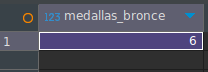
\includegraphics[width=10cm]{resources/resultados/r8.png}
\end{center}   

Nota: Para este resultado, tambien se añadieron manualmente tuplas en la tabla Medalla. \vspace{.3cm}